\chapter{Results}\label{ch:results}
This chapter will give an overview of the results of the tests performed on the system.

\section{Stationary test}\label{sec:stationary-test}
The stationary test is a test to determine the measurement noise of the sensors.
The test is done by placing the sensors in a stationary position, and measuring the noise of the sensors.
A plot of the measured latitude and longitude can be seen in Figure~\ref{fig:stationary-test}.

\begin{figure}[H]
    \centering
    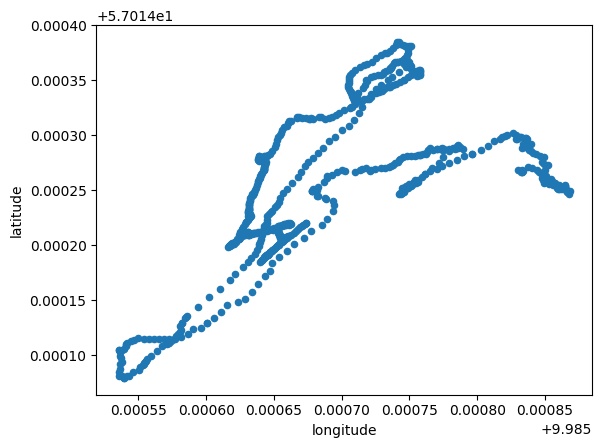
\includegraphics[width=0.8\textwidth]{chapters/05Results/figures/output}
    \caption{Plot of measured values from the stationary test.}
    \label{fig:stationary-test}
\end{figure}
It is noted that the latitude and longitude does not appear to be influened by white noise, as the values are not jumping around but rather moving in a smooth manner.

A plot of the measured altitudes from the pressuresensor and the GPS module can be seen in Figure~\ref{fig:altitude-test}

\begin{figure}
    \centering
    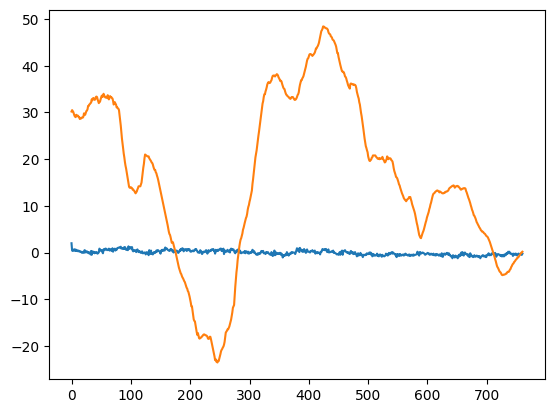
\includegraphics[width=0.8\textwidth]{chapters/05Results/figures/altitude}
    \caption{Plot of measured altitudes from the stationary test.}
    \label{fig:altitude-test}
\end{figure}

It is noted that the GPS altitude is also not influenced by white noise.

From this test the variance of the measurement noise of the sensors is found to be:
\begin{align}
    \sigma_{\text{latitude}} &= 4.95\mathrm{e}-09\nonumber\\
    \sigma_{\text{longitude}} &= 6.169\mathrm{e}-09\nonumber\\
    \sigma_{\text{gps\_altitude}} &= 322.83\nonumber \\
    \sigma_{\text{gps\_altitude\_v}} &= 1.406 \nonumber\\
    \sigma_{\text{pressure\_altitude}} &= 0.248 \nonumber\\
    \sigma_{\text{pressure\_alt\_v}} &= 0.0989\nonumber\\
    \sigma_{\text{v\_lat}} &= 0.0\nonumber\\
    \sigma_{\text{v\_long}} &= 0.004217 \nonumber
\end{align}
These values is used as the measurement noise in the Kalman filter.
The process noise is set to 1e-8 for all states.

\section{Kalman filter test}\label{sec:kalman-filter-test}
In this test the Kalman filter is tested.
Due to time constraints, the test is done on the stationary data from the stationary test.
It can however be seen that the Kalman filter is able to filter out the noise from the sensors, and combine the multiple sensors to a more accurate estimate.
A plot of the estimated altitude can be seen in Figure~\ref{fig:kalman-filter-test}.

\begin{figure}[H]
    \centering
    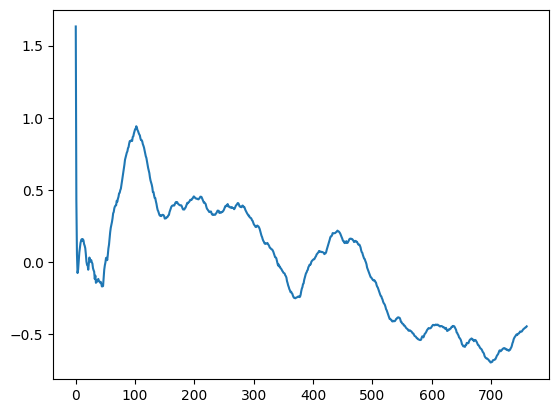
\includegraphics[width=0.8\textwidth]{chapters/05Results/figures/filtered_alt_only}
    \caption{Plot of the estimated altitude from the Kalman filter.}
    \label{fig:kalman-filter-test}
\end{figure}

Comparing the output to the measured altitude of both the GPS module and the pressure sensor, it can be seen that the Kalman filter almost only outputs the pressure sensor data.
This is due to the fact that the pressure sensor has a much lower variance than the GPS module.
This can be seen in Figure~\ref{fig:kalman-filter-test-compare}.
\begin{figure}[H]
    \centering
    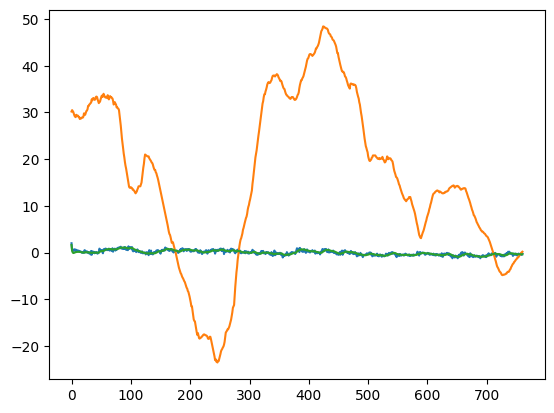
\includegraphics[width=0.8\textwidth]{chapters/05Results/figures/filtere_pres_gpsalt}
    \caption{Plot of the estimated altitude from the Kalman filter compared to the measured altitude.}
    \label{fig:kalman-filter-test-compare}
\end{figure}

By not plotting the GPS altitude, the output of the kalman filter can better be seen.
This can be seen in Figure~\ref{fig:kalman-filter-test-compare-no-gps}.
\begin{figure}[H]
    \centering
    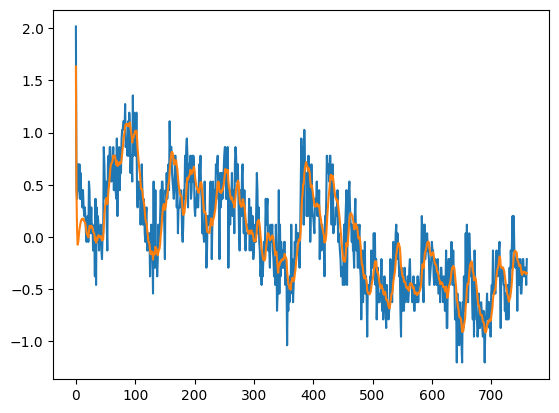
\includegraphics[width=0.8\textwidth]{chapters/05Results/figures/filtered_state_bar_alt}
    \caption{Plot of the estimated altitude from the Kalman filter compared to the measured altitude.}
    \label{fig:kalman-filter-test-compare-no-gps}
\end{figure}

The filtered latitude and longitude can be seen in Figure~\ref{fig:kalman-filter-lat-long}.
\begin{figure}[H]
    \centering
    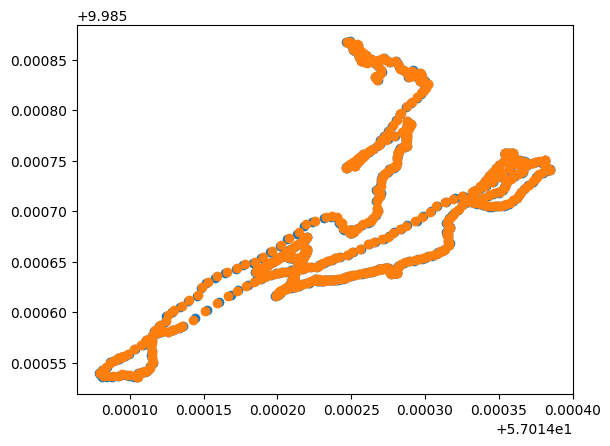
\includegraphics[width=0.8\textwidth]{chapters/05Results/figures/lat_long_filtered}
    \caption{Plot of the estimated latitude and longitude from the Kalman filter.}
    \label{fig:kalman-filter-lat-long}
\end{figure}

As it can be seen from the plot, there is not much difference between the filtered and the measured values.



